\texttt{placeholder abstract - only for general idea not to be proofread}
\smallskip

\begin{figure}
    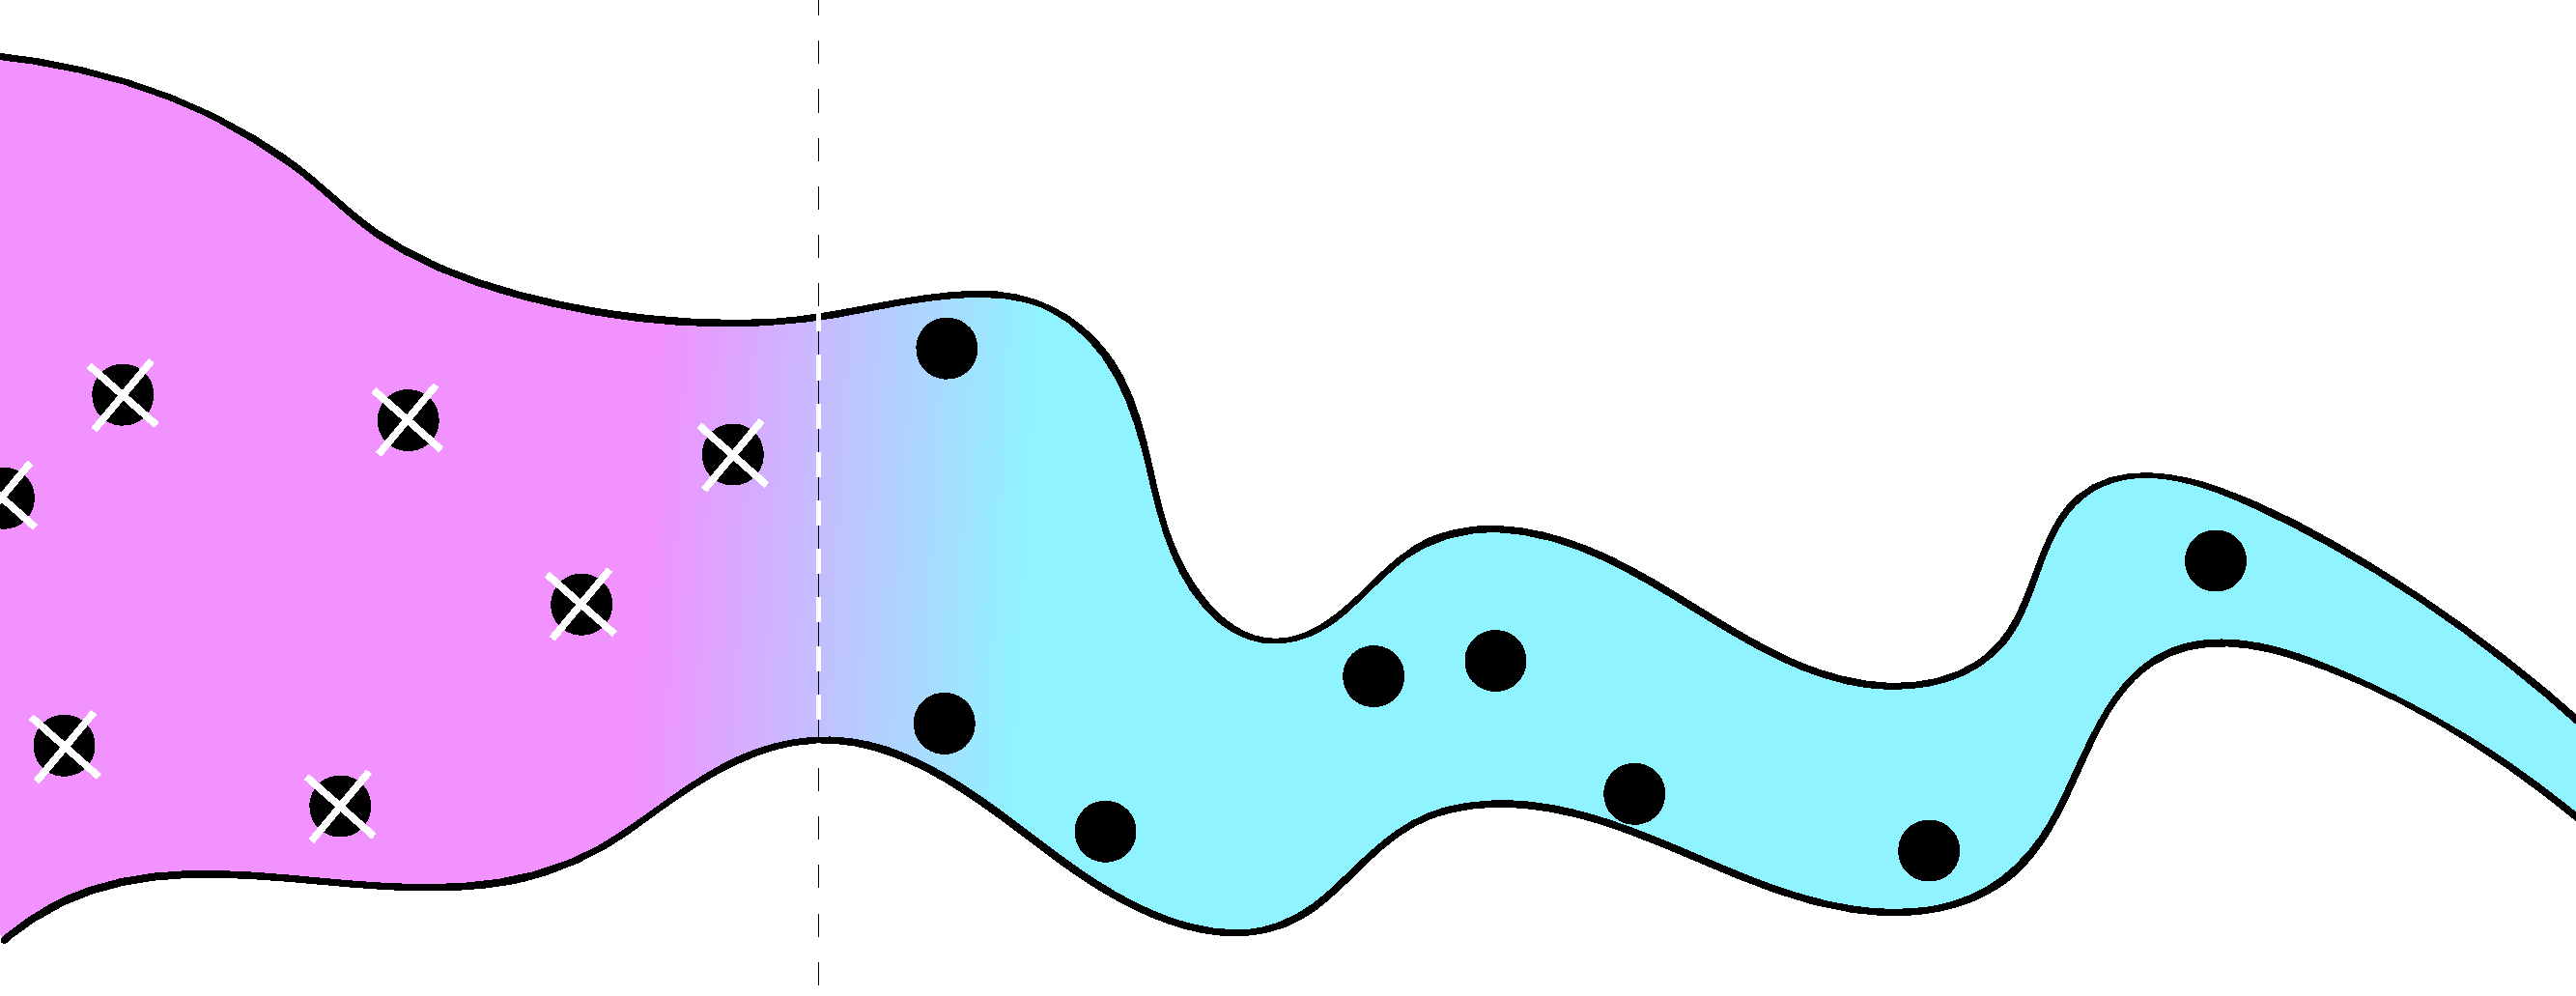
\includegraphics[width=\columnwidth]{picto visual abstract.pdf}
\end{figure}
Estuaries are a challenging for plankton.
Gradients are steep and currents are strong.
Retention mechanisms crucial process for survival.
However, very little experimental and theoretical evidence has been gathered.
We will conduct a model study.
First we will show the importance of retention mechanism for plankton in the Elbe.
Secondly we will study different retention mechanism which are suspected to be applied by organism.
We compare the outcome of the different experiment and judge their effectiveness.

\section*{Introduction}

\texttt{All texts in this old fashioned typewriter fonds are comments and thoughts on the texts and not part of the actual paper.}
\smallskip

\subsection*{Estuaries and Phytoplankton}

\texttt{In this section I try to convey: why we care about estuaries and why we focus on phytoplankton and illustrate why question "How does Phytoplankton retain itself in an estuary?" is interesting.}


\textbf{Estuaries are important} both for the climate system as well as important human habitat.
From a climate perspective they offer a high productivity relative to surface area which results in large amounts of direct carbon cycling as well as their important role as a source of nutrients and hatching grounds for marine ecosystem.
From a human habitat role they offer easy access to marine ecosystem while still providing fresh water.
Hence, "key human hatching grounds"

Complex ecosystem: Both marine and freshwater influence, complex topology and hydrodynmics, strong antropogenics make it hard to study and many open questions remain to this day.
In this study we will take a look at phytoplankton and its mechanism to retain itself in the estuary.

The aquatic part of the ecosystem is strongly controlled by \textbf{phytoplankton} because in its role as a primary producer it acts as prey for most higher trophic levels (cite)
However phytoplankton as all planktonic organism drift in the current. Due to the current in the estuary we expect plankton to be drifting downstream over time and ultimately be washed out into marine high salinity waters.
Hence, we wonder how phytoplankton manages to survive as a populating in such an environment.
Assuming the population is not exclusively maintained by upstream plankton that is washed into the estuary. Then there must be some sort of retention mechanism that enables phytoplankton to not be washed out.
While this is expected to be an crucial mechanism for survival it is currently not well understood due to the difficulty in either measuring or modeling such processes.


\subsection*{Previous studies - aka - what is known}

\texttt{In this section I try to outline what is known and use it to illustrate the research gap}
\smallskip

We categorize the already performed studies on the subject of phytoplankton retention in three groups: observations, theoretical- and realistic-modelling studies.

\textbf{Observational} studies have found three major mechanism for retention - diel migration, sinking and stickiness.
Diel migration has been found - moving verticaly up and down with the sun - but only in larger organisms which are not strictly planktonic (fish-larve, mesozooplanktion) [cite]
Also bentic plankton has been observed that is strongly negativly buoyand aka sinking and sticking to the ground

Here we want to highlight two \textbf{theoretical} studies studying the mechanisms of "loss compensation" and "reseeding".
(cite) theorized a set up in which they  a population is able to maintain itself if the losses due to outwashing can be compensated by growth (cite).
In a setup where a lake system was modelled they were able to quantify reproductino thersholds that are needed to maintain the population.
However, this setup also implies that the growing part of the population is somehow retaining their position.
If the regrowing population is also continuously drifting downstream they will also ultimately die out.

(cite) studied the concept of "reseeding".
Here a system is theorized in which a population is able to repopulate an previsouly uncolonized area upstream due to local upstream eddies.
While they showed that upstream reseeding is conceptually possible they did so in an contrived system.

\smallskip
\texttt{More detail?}
\smallskip

Hence, it has been showed both "outgrowing the losses" and "reseeding" are possible retention mechanism but only under certain conditions.



In (cite) they use a \textbf{particle tracking model} also known as Lagragian model to study Zooplankton movement in the San Francisco Bay.
They were able to show  that sinking and diel migration slows the outwashing process and might be beneficial retention tactic
However, they did so by ignoring key processes like reproduction and death in an rectangular grid model which further introduces some numerical problems.


To \textbf{summarize} - several concepts for potential retention mechanisms have been found and shown to work in certain conditions.
However, all approaches used major simplification which didn't allow them to study the full picture.
We developed a new and more realistic approach to study retention with an particle tracking model combining many of the above outlined features into one model.

\section*{Methods}

\subsection*{general model description}

In our study we take a particle tracking approach with a \textbf{lagrangian model} called Oceantracker (cite).
Particle tracking offers several advantages for our question:
While particle tracking on unstructured grids is relatively computationally expensive it allows us to reuse already validated hydrodynamic models. Which is overall still much faster then using concentration based models.
Because we are tracking particles we can observer their individual tracks which makes it easier to interpret (plankton is particle)
It also allows us to include "individual based processes" (not really used currently)
But most importantly it allows us for a better representation of the behavior close to the edges of the estuary. (100m boxes in concentration based models)
\begin{figure}
    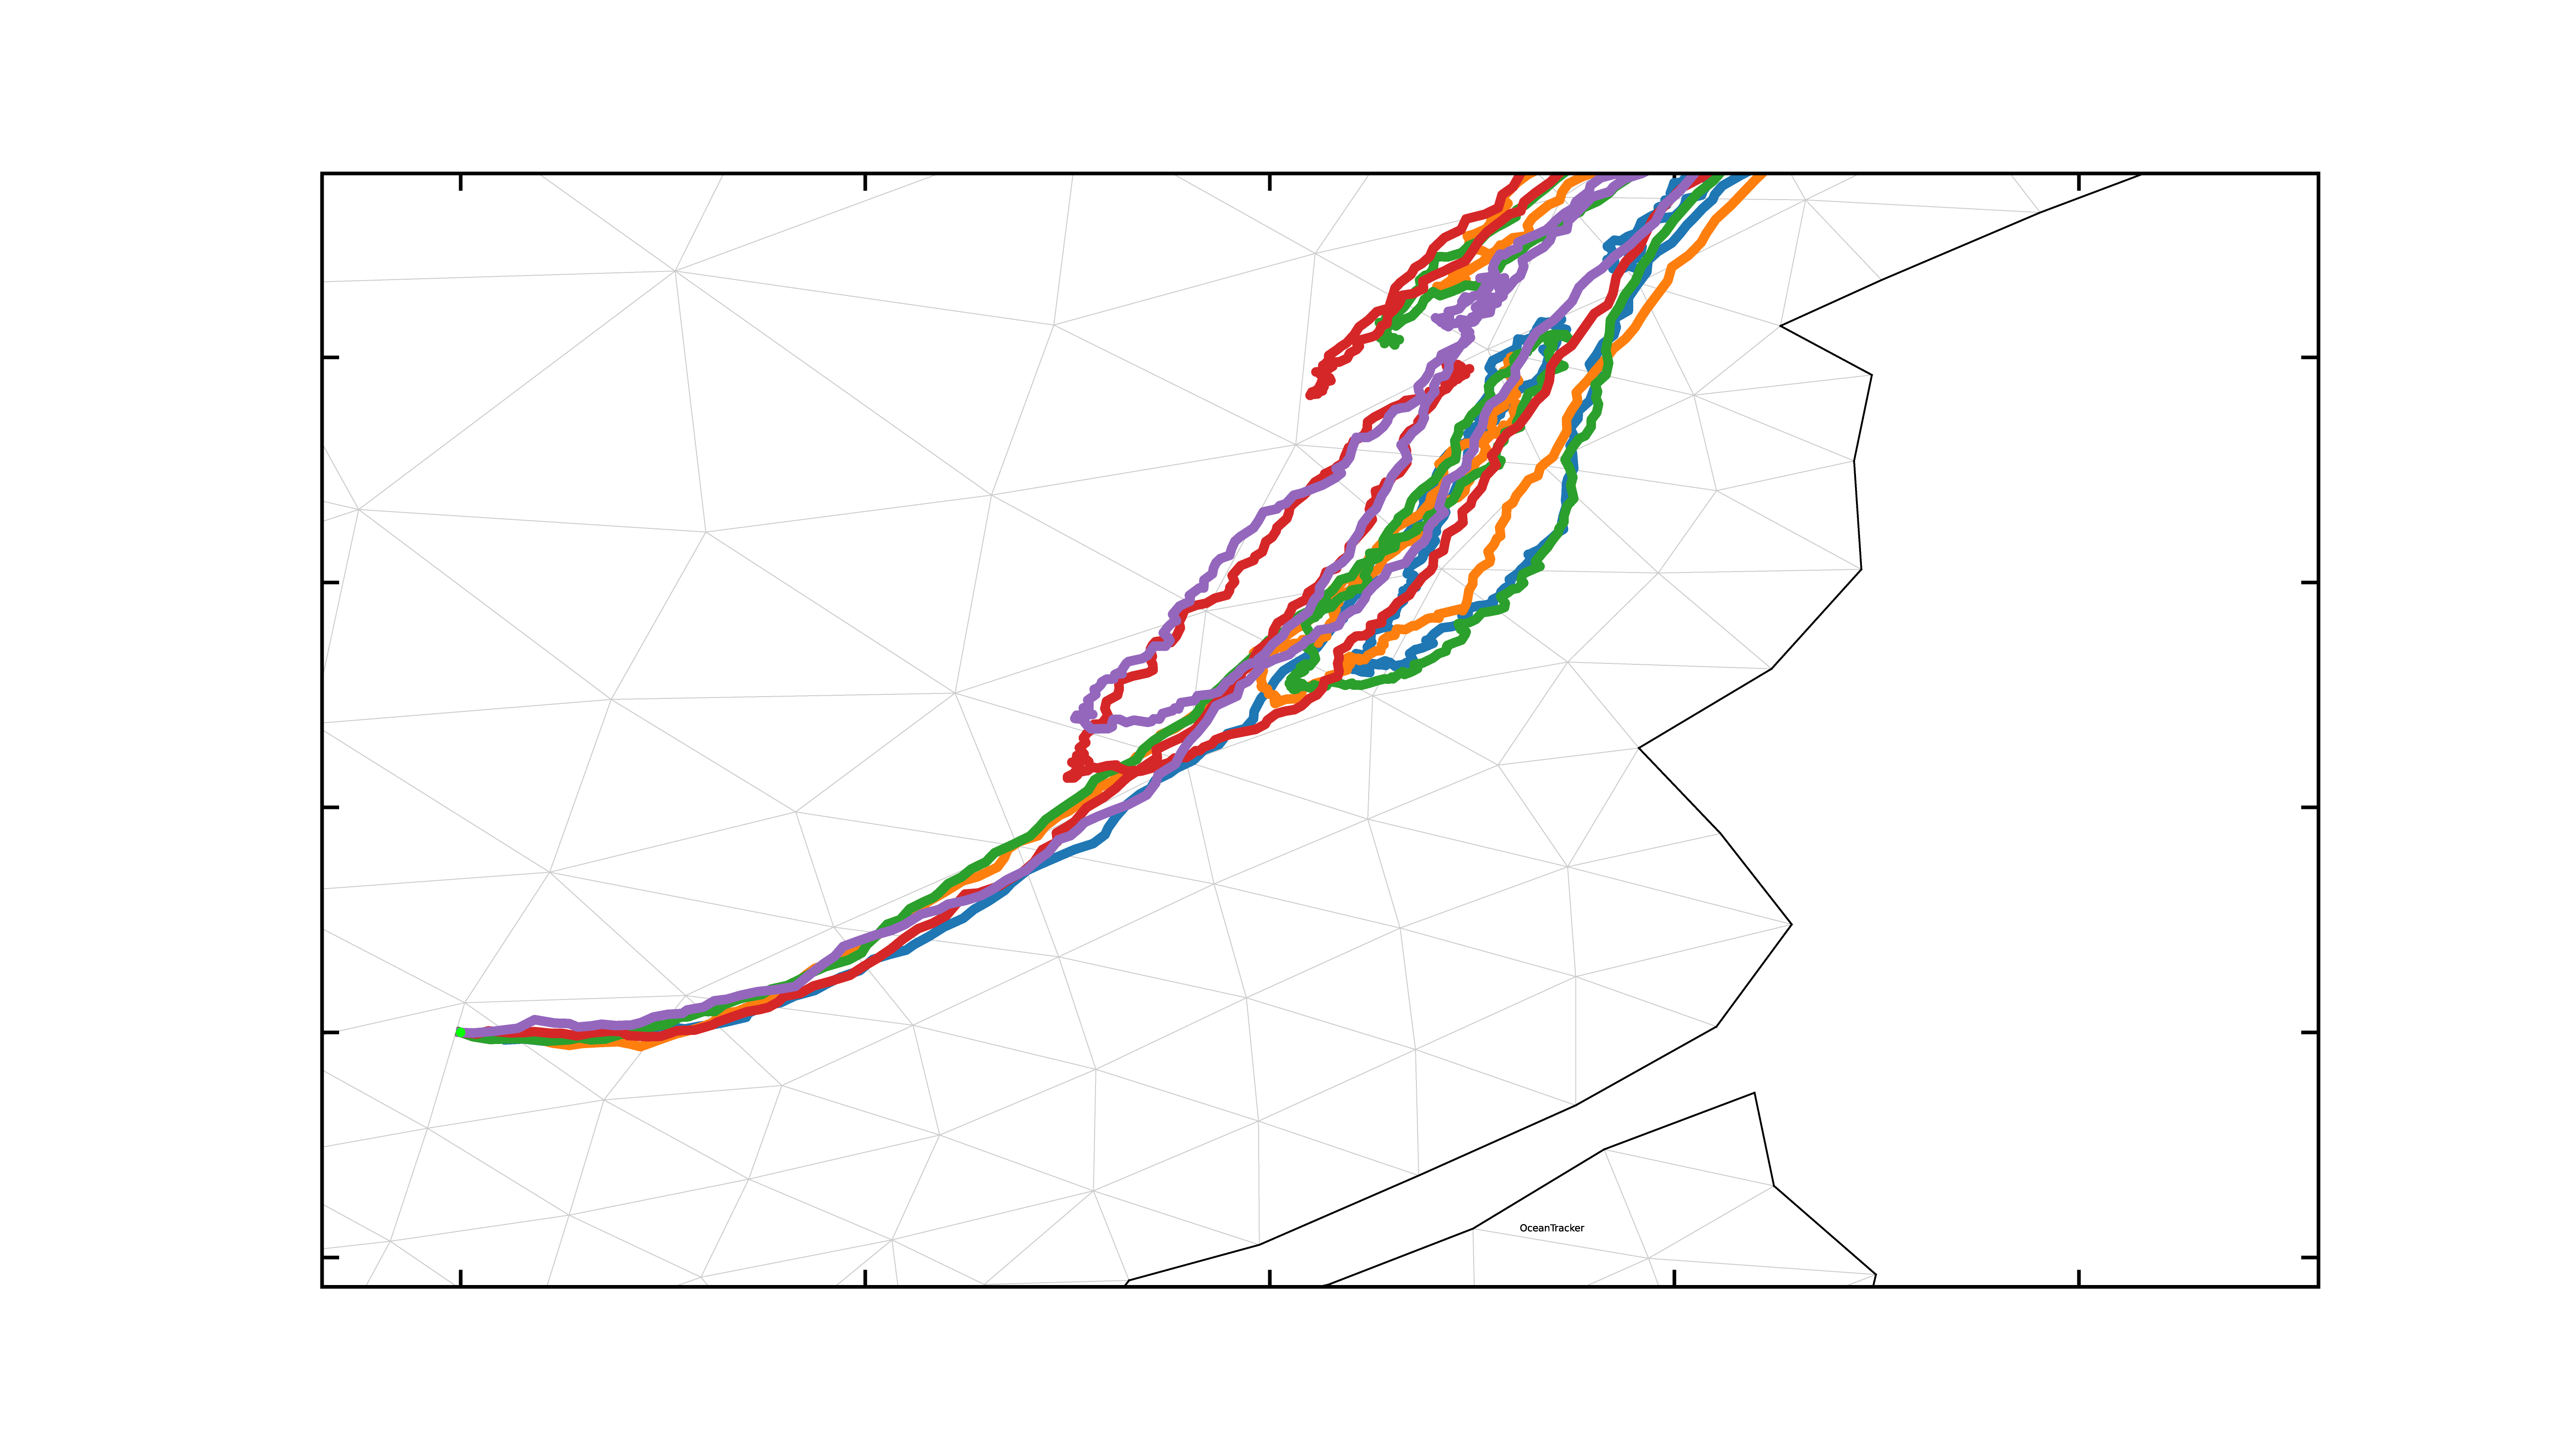
\includegraphics[width=\columnwidth]{Artboard 2.png}
    \caption{Particle Trackle visualisation - particle tracks on grid}
\end{figure}

\textbf{data}
The hydrodynamics are taken from a SCHISM model from a Johannes Pein (cite) 
It is an three dimensional unstructured  grid model representing the full estuary from the weir at geesthacht close to helgoland including side-channels and the harbor area.
(Look for more details in pein paper that might be interesting)
It provides a node-based mesh field containing a range of information.
For our purpose the water velocities represented in a flow field is the most important one
But also salinity and many other more technical information is used (meh)
We study the year 2012 with 1h temporal- and dynamically varying spacial resolution.

\begin{figure}
    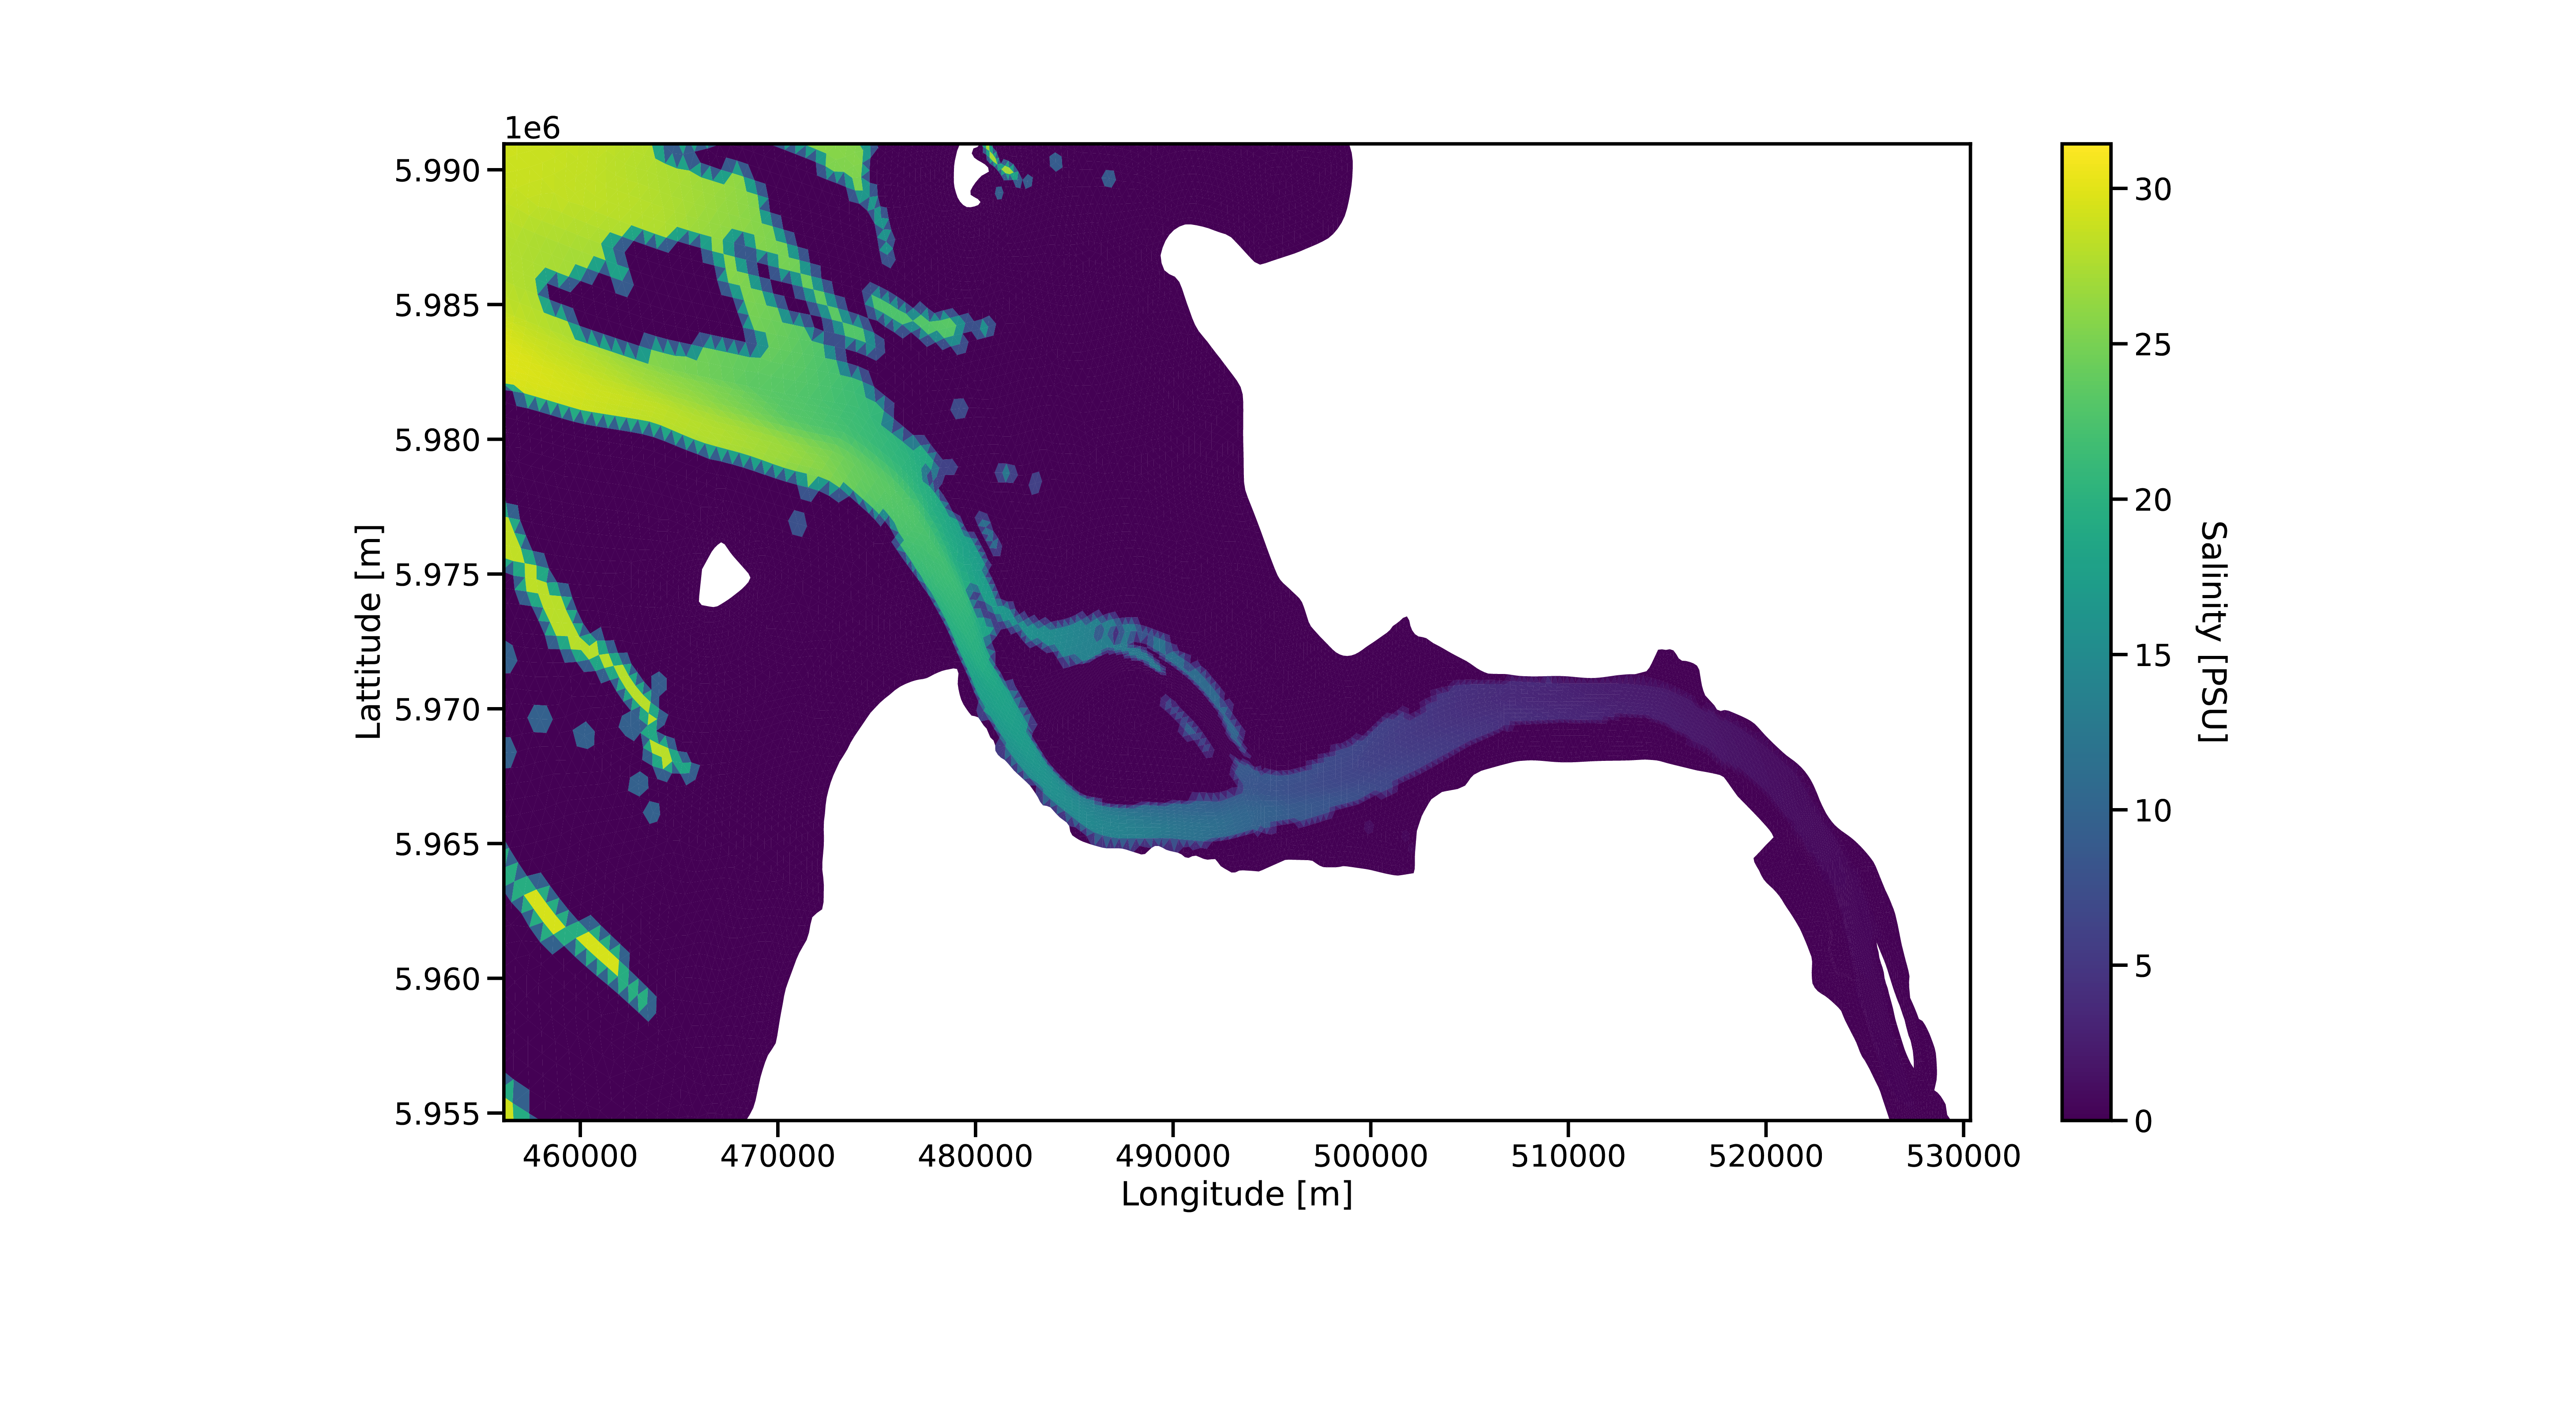
\includegraphics[width=\columnwidth]{Artboard 1.png}
    \caption{model domain visualization - full range grid including statistical polygons for later reference and example of a scalar field (e.g. temperature)}
    \label{fig:statistial polygons}
\end{figure}

\textbf{bio-logical mechanisms represented in the model}
On top of the "blanc" particle we add a set of biological features to achieve a more realistic behavior.
The most important one is their ability to reproduce by creating copies of themselves and their ability to die in certain conditions.
We also add a set of movement related features. This includes a vertical movement behaviour. We included constant verticle velocities aka sinking and rising and a time dependent one namely diel-migration.
Their interaction with the boundaries of our model is represted by a simple sedimentation and resuspension model in the water and a stranding model on land

% \begin{figure}
%     \centering
%     \begin{minipage}{.4\columnwidth}
%         \centering
%         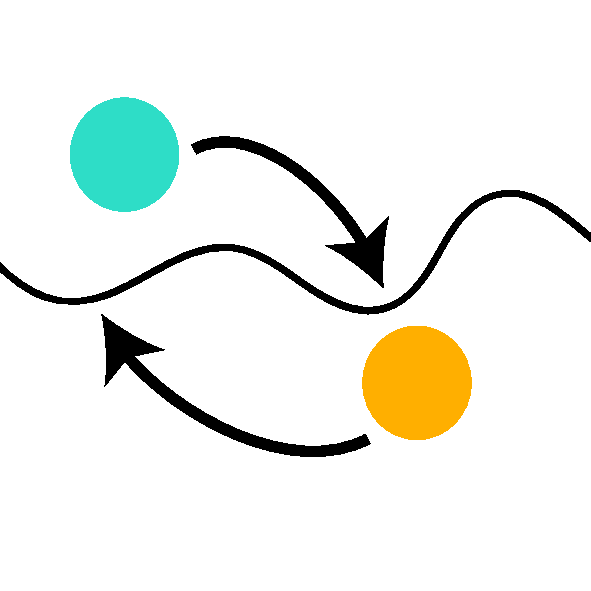
\includegraphics[width=.3\columnwidth]{picto resuspension.pdf}
%     \end{minipage}
%     \begin{minipage}{.4\columnwidth}
%     \centering
%         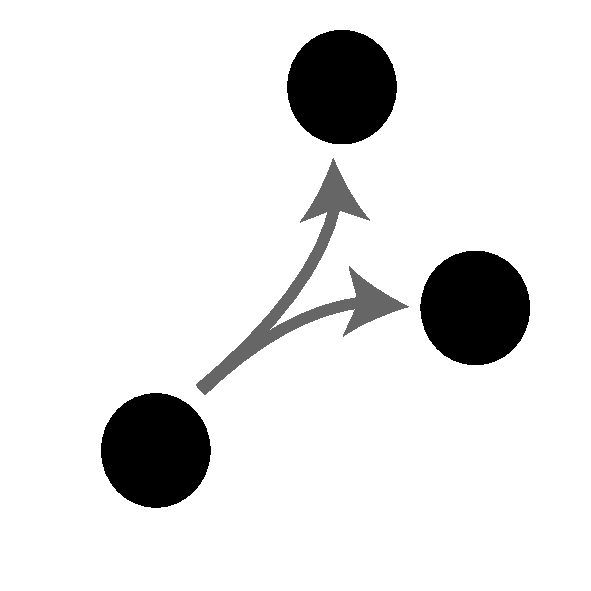
\includegraphics[width=.3\columnwidth]{picto splitting.pdf}
%     \end{minipage}
%     \caption{examples of pictograms for bio processes}
% \end{figure}



% \begin{figure}
%     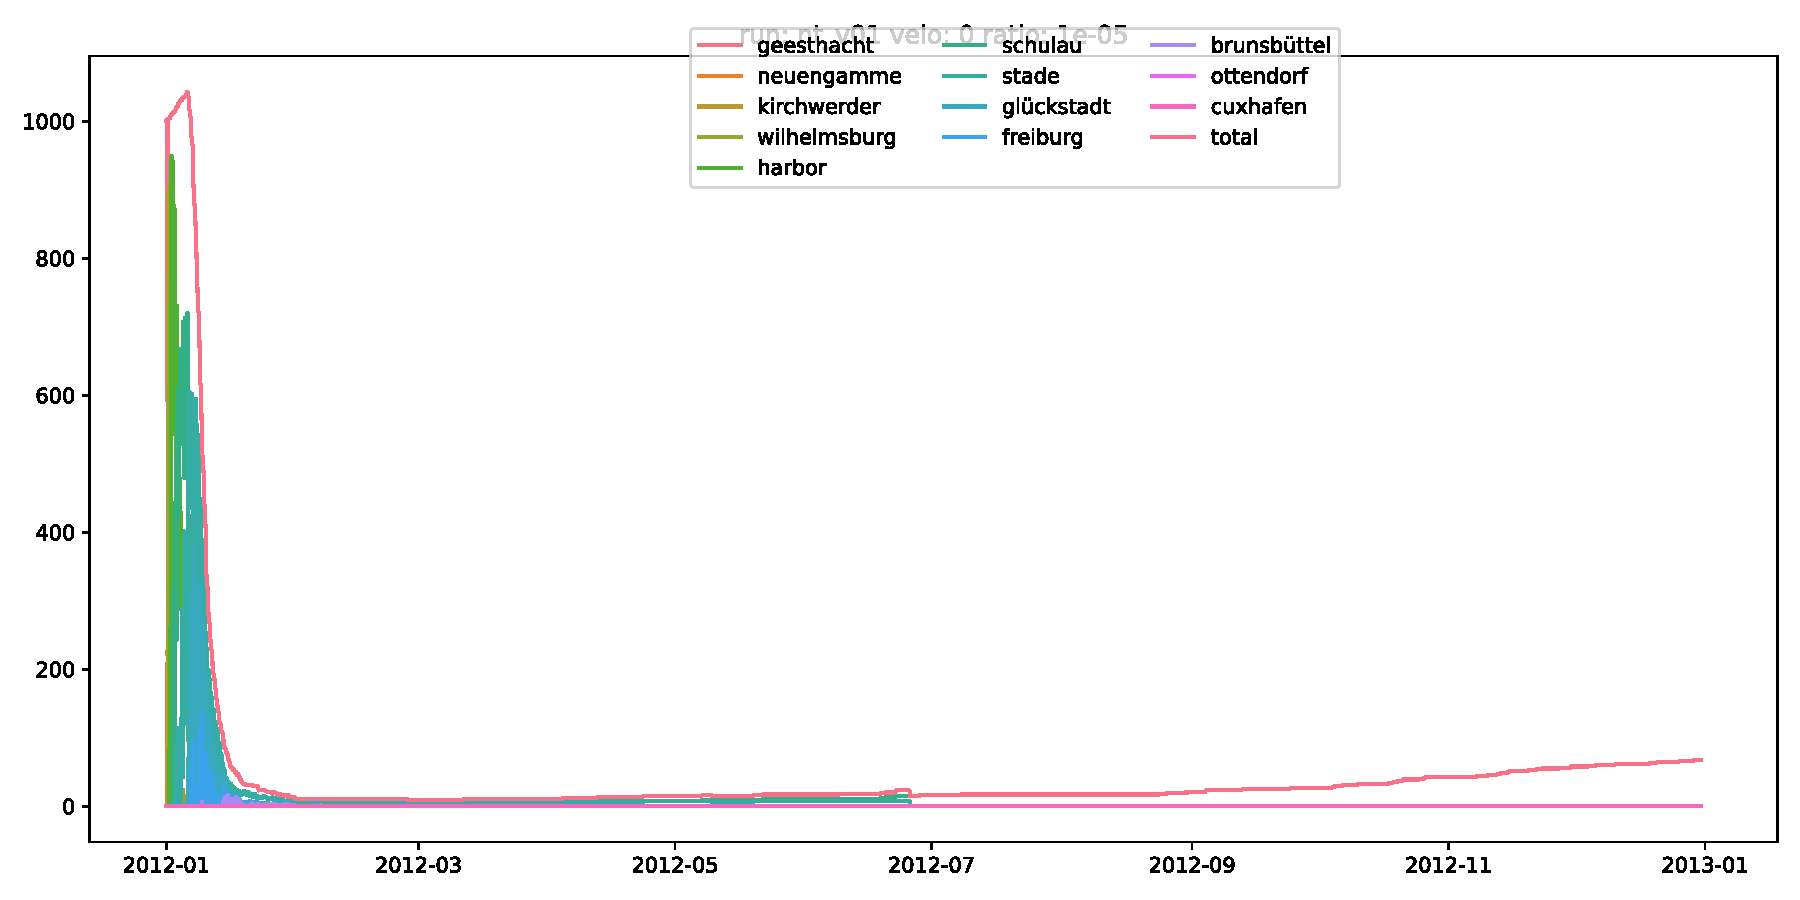
\includegraphics[width=\columnwidth]{fixed_particle_culling.pdf}
%     \caption{Example 2d plot of particle counts, centroid and "retainment" threshold}
% \end{figure}

\subsection*{Experimental configurations}

% \begin{figure}
%     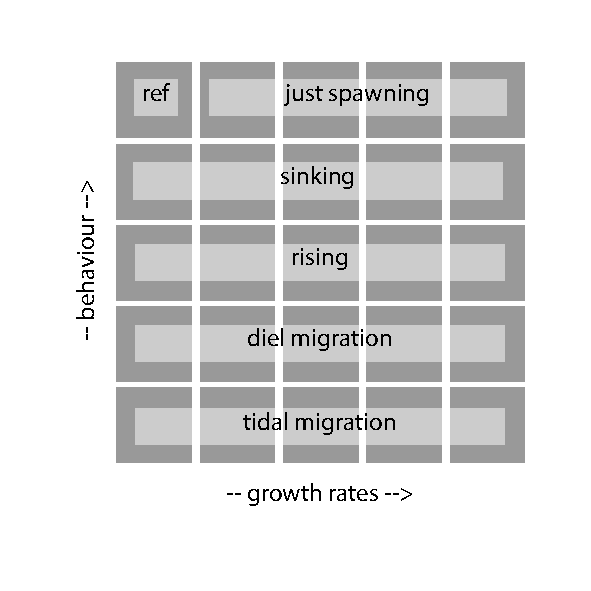
\includegraphics[width=\columnwidth]{plot experimental configuration.pdf}
%     \caption{2d grid with boxes for the different cases/dimension. 
%              Same structure as the later sensitivity analysis plot used \ref{fig:retention_results_SA}}
%     \label{fig:experimental_configuration}
% \end{figure}


\textbf{downstream retention}
The first and major experiment of this studies examines retention mechanisms under different scenarios.
General idea is to release a population of plankton at the weir in geesthacht and examine how the population distrubutes itself over the estuary and whether it is able to maintain its population size.
We examine the effect of several mechanism. These include:
\textit{Reproduction} represented as a chance of duplicating a particle,
\textit{vertical migration} where two modes have been implemented. A constant up or downward drift and diel migration where the drift speed and direction is based on the phase of the sun.
Particles can \textit{strand and resuspend} from the shore when the water level rises again.
They can also \textit{sink and suspend} on the bottom and resuspend based on a critical-friction-velocity concept.
Particles are removed if they either reach high salinity waters implemented as a mortality chance above $10 PSU$,
when they are stranded until they dry out which is represented by killing all particles which have not been rewettet in the last $7$ days,
and when they are starved for light which we defined as removing all particles which have been in low-light areas longer then a total of $14$ days where presence in high-light areas is subtracted from the starvation budget.
\texttt{Hallo, mein Name ist Kleist.}
The model also implements dynamic dispersion that is crucial to represent tidal-pumping processes and to allow for a realistic trajectories close to boundaries.

\smallskip
\texttt{More detail needed? - or should that go into the appendix?}
\smallskip

The observed particle batch representing out phytoplankton population is released at new years eve in a volume at the weir in Geesthacht which marks the beginning of the Estuary.
We evaluate their \textbf{retention success} primarily by measuring the amount of plankton in different regions in the estuary over time.
If the population survives a full year and its population is over a certain threshold we consider them "successfully retainted".

To count the particles we use "\textbf{statistical polygons}".
We use to split the estuaries in along-shore section. See  \ref{fig:statistial polygons}
\texttt{Well, actually we don't really use the individual polygons in any of the metrics but only for debugging and visualization purposes. Are they interesting anyway?}

We also log their distance traveled, age, water depth, and status - whether they are drifting, stranded on the shore or bottom.
This allows us to compare the successful (died old) and unsuccessful (died young) particles 
The logged observables are measured every 12 hours and include location, status, water level, age, distance traveled  

We use this set-up in a range of scenarios and compare them to each other.
We call the first and simples scenario "dust". Here we don't allow for any reproduction and give all particles a neutral buoyancy.
This is our reference for any retention strategy. Any beneficial strategy must perform better then these passive tracers.

In the second scenario - referred to as "migrating" - re-enable reproduction and also give the particles a range of different buoyancies resulting in positive, negative or in the case of the diel-mirgrating particles oscillating vertical velocities.
We also allow reproduction with a range of different growth rates.

The third scenario has been added for illustration purposes.
Here, we use the same set-up as in the second scenario with the only exception of disabling reproduction for particles stranded on the shores of the estuaries.
We call this scenario "waiting-for-resuspension"
\label{txt:waiting-for-resuspsension}
But more on that later.

The tested parameters described above like reproduction and vertical movement can be found in table \ref{tab:downstream_retention_params}.
\smallskip
\texttt{The table doesn't exist yet.}
\smallskip


\section*{Results}

\subsection*{Retentions experiments}

\subsubsection*{Scenario: "dust"}: 
\begin{figure}
    \includegraphics[width=\columnwidth]{example-image-a}
    \caption[]{total particles counts for scenario "dust" for all tested parameters}
    \label{fig:dust_particle_counts}
\end{figure}
In fig \ref{fig:dust_particle_counts} the particle counts measured over time it the estuary are shown.
We can clearly see that the total particle count drops to zero - in most cases already after less then two months.
From this we deduce that particles are constantly getting washed out and do not find "sheltered areas" in which they can remain for a long time.
This also means that reproduction is a necessary condition for the population to maintain their population even if all mortality sources except high-salinity are ignored.


\subsubsection*{Scenario: "migration"}: 
\begin{figure}
    \includegraphics[width=\columnwidth]{example-image-a}
    \caption[]{total particles counts for scenario "migration" with a monotonic migration pattern for all tested parameters}
    \label{fig:monotonic_particle_counts}
\end{figure}
\begin{figure}
    \includegraphics[width=\columnwidth]{example-image-a}
    \caption[]{total particles counts for scenario "migration" with a diel migration pattern for all tested parameters}
    \label{fig:diel_particle_counts}
\end{figure}

In fig \ref{fig:monotonic_particle_counts} and \ref{fig:diel_particle_counts} we can see that the population manages to maintain themselves in certain conditions.
The fact that we found conditions for survival in this simplistic setup is in itself interesting for two major reasons.
First, all previsous studies implementing a phytoplankton in an Elbe model required constant reseeding either up and/or downstream.
Hence, we are the first study that is able to provide an estimate for the conditions necessary for "in-estuar"-survival.

\texttt{ The secondly might be better suited for the discussion.}

Secondly, while we assume ad libitum nutrient conditions for the phytoplankton we do not implement any sub-grid-resolution structure on the shores.
Hence, the river banks are perfectly flat sand banks without vegetation which might aid the retention of phytoplankton.

\texttt{Add comparison of monotonic upwards to downwards, monotonic to diel, and the discuss the relative growth rate thresholds}

Lets now take a closer look at the subset of pytoplankton that was able to retain themselves compared to those getting washed out.
We divide the population now into a long-living and short-living set with an threshold age of 3 months.
We compare these two sets now by their water depth, distance traveled, and ratio of time stranded to drifting.
You can see these measurement visualized in the boxplots \ref{fig:migration-long-vs-short}

\begin{figure}
    \includegraphics[width=\columnwidth]{example-image-a}
    \caption[]{Boxplot of long-vs-short showing water depth}
    \label{fig:migration-long-vs-short}
\end{figure}

We can consistently see that the long living subset is in shallower water, does move less, and is a significantly longer stranded then drifting.
In fig. \ref{fig:migration-long-vs-short-heatmap} we show the special distribution of the long- and short-living subset.

\begin{figure}
    \includegraphics[width=\columnwidth]{example-image-a}
    \caption[]{heatmap of long-living to short-living-particles}
    \label{fig:migration-long-vs-short-heatmap}
\end{figure}

\texttt{show zoom in with water depth?}

\subsubsection*{Scenario: "waiting-for-resuspension"}

\begin{figure}
    \includegraphics[width=\columnwidth]{example-image-a}
    \caption[]{total particles counts for scenario "waiting-for-resuspension" with a monotonic migration pattern for all tested parameters}
    \label{fig:stranded-monotonic-particle-counts}
\end{figure}
\begin{figure}
    \includegraphics[width=\columnwidth]{example-image-a}
    \caption[]{total particles counts for scenario "waiting-for-resuspension" with a diel migration pattern for all tested parameters}
    \label{fig:stranded-diel-particle-counts}
\end{figure}

In fig \ref{fig:stranded-monotonic-particle-counts} and \ref{fig:stranded-diel-particle-counts} we again see the total particle counts.
Keep in mind that the only difference in the model configuration to the "migration" run is that phytoplankton growth has been disabled when the plankton is stranded.
We can clearly see that phytoplankton dies out in these conditions for the full parameter space.
From this we deduce that the shallow areas are not only crucial for improved retention but also a necessary hatching ground.

To summarize the retention experiments: We saw that the population is ultimately washed out and perishes if we surpress reproduction.
We also saw that with reproduction phytoplankton is able to maintain their population strain without up- or downstream reseeding under certain conditions!
In the last experiment we showed that the shallow water areas are not only helpfull but crucial for the survival of the population.

\textbf{upstream migration}
\begin{figure}
    \includegraphics[width=\columnwidth]{example-image-a}
    \caption[]{particle counts in upstream statistical polygons}
    \label{fig:upstream-migration-statistical-poly-counts}
\end{figure}
As previsouly described - In the upstream migration experiment we divide the estuary in short ($\sim 50km$) sections.
We release particles in all of these sections and count their occurence in other sections.
In fig \ref{fig:upstream-migration-statistical-poly-counts} the particle counts for the two upstream sections from the release location.
We consider upstream migration to happen when plankton moves two sections up and is able to retain itself there.
\texttt{Do I need to explain why two polygons and why being there only briefly won't work?}

\texttt{No results yet with the proper dispersion model. In the previous run upstream migration did not occur and was considered to be a negligible mechanism in the retention process.}



\section*{Discussion}
\texttt{The discussion is currently only a list of bullet points that I considered to discuss so far. It is by no means complete or currently not worth reading.}
\begin{itemize}
    \item discuss limitation of the model
    \begin{itemize}
        \item simplified bottom/sediment interaction
        \item no "small object" representation e.g. vegetation or "rocks" $\rightarrow$ implices underestimation of "retention"
        \item simplistic bio representation. does not allow for precise quantification but only indicates bounds aka "even in ideal conditions they couldn't survive if ..."
        \item other minor issues - temporal resolution, particle out-of-bounds cases etc
        \item discuss choice of particle tracking model compared to concentration based model
    \end{itemize}
    \item conclusions that we draw from this:
    \begin{itemize}
        \item from a population-surival perspective the plankton that does not drift to shallow water are "dead man walking" as all decendents of these particles will ultimately die.
        \item we need cross-shore sampling to better understand this. currently all specially resolved sampling strategies are along shor - aka in the center of the river
        \item shallow water is crucial for the survival. hence the protection and restoration of shallow regions is crucial for ecosystem healthiness
    \end{itemize}
\end{itemize}